\newpage
\chapter{ANEXOS}
%\addcontentsline{toc}{chapter}{ANEXOS}
\newpage
%\phantomsection
\section{PLAN DE GESTIÓN DE RIESGOS}\label{sec:plan-riesgos}
%\addcontentsline{toc}{section}{PLAN DE GESTIÓN DE RIESGOS}
La gestión de los riesgos consiste en la identificación de los riesgos y la planificación para minimizar su efecto en el proyecto. Siguiendo la metodología del PMBOK \cite{PMBOK}, se define una gestión compuesta por los siguientes pasos:
\begin{itemize}
\item Planificar la Gestión de Riesgos.
\item Identificar los riesgos.
\item Realizar el análisis cualitativo de riesgos.
\item Realizar el análisis cuantitativo de riesgos.
\item Planificar la respuesta a los riesgos.
\item Monitorizar y controlar los riesgos.
\end{itemize}
A continuación se describirán los conceptos necesarios para planificar la gestión de riesgos, ya que los siguientes pasos se habrán realizado en la sección \ref{sec:riesgos}
\paragraph*{Categorías de riesgos}
Se categorizan los riesgos según la siguiente estructura de desglose:
\begin{figure}[H]
\centering
\centerline{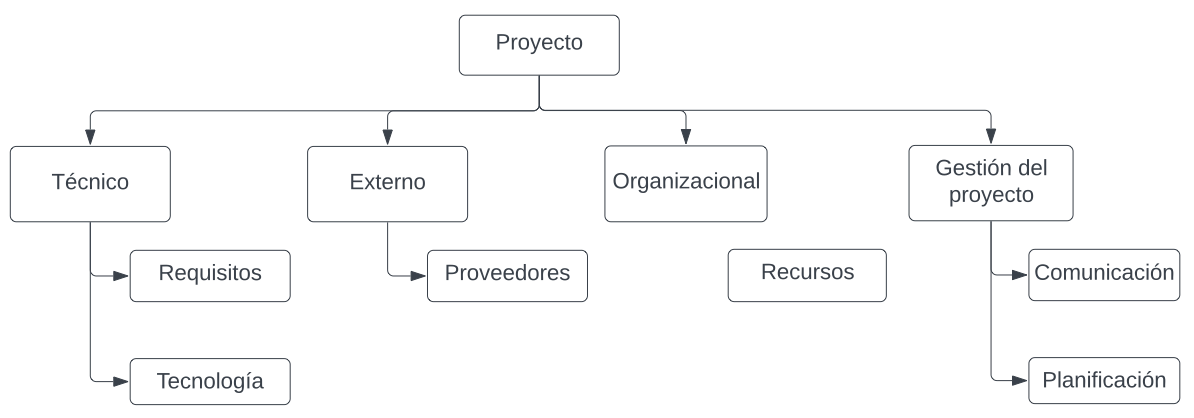
\includegraphics[scale=0.5]{rbs}}
\caption{Risk Breakdown Structure}
\end{figure}

\paragraph*{Probabilidad e impacto}
Se deben priorizar los riesgos de un proyecto en función de su prioridad de ocurrencia e impacto. A continuación se muestra la definición de las probabilidades y las escalas de impacto para riesgos negativos.
\begin{figure}[H]
\centering
\centerline{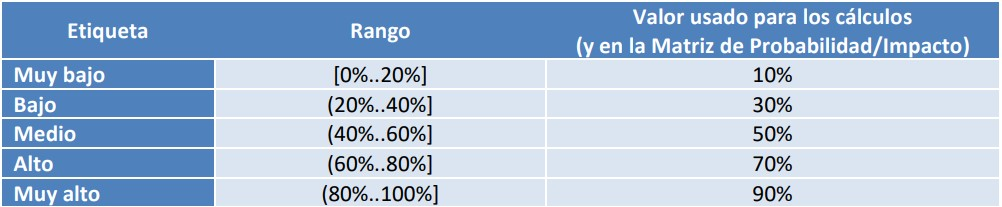
\includegraphics[scale=0.6]{def-probabilidades}}
\caption{Tabla de definición de probabilidades}
\end{figure}
\begin{figure}[H]
\centering
\centerline{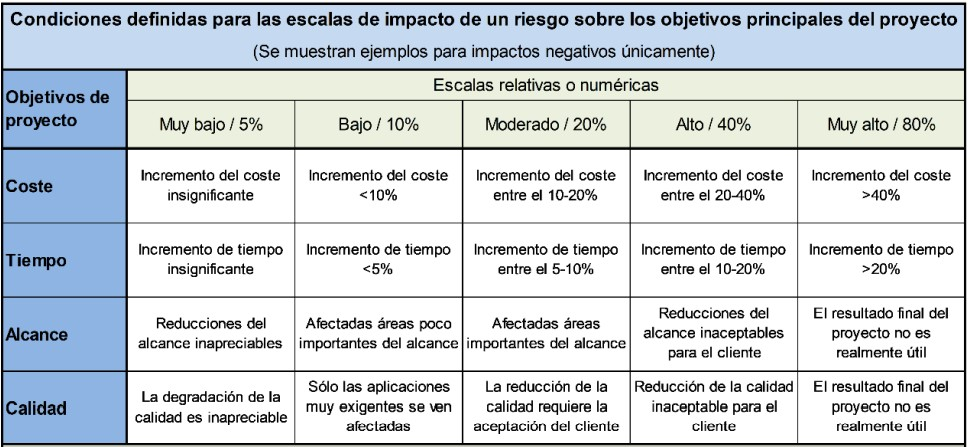
\includegraphics[scale=0.6]{escalas-impacto}}
\caption{Escalas de impacto sobre los objetivos del proyecto}
\end{figure}

\paragraph*{Matriz de probabilidad e impacto}
Esta matriz define los valores usados para priorizar los riesgos.
\begin{figure}[H]
\centering
\centerline{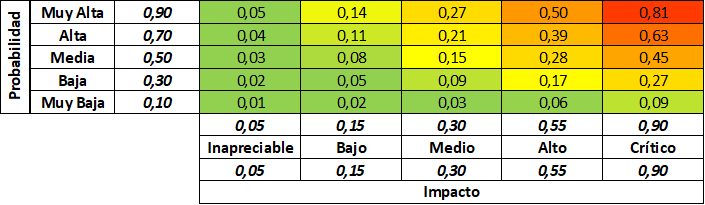
\includegraphics[scale=0.8]{matriz-prob}}
\caption{Matriz de Probabilidad e Impacto}
\end{figure}


\newpage
\section{CONTENIDO ENTREGADO EN LOS ANEXOS}\label{sec:contenido_anexos}
%\addcontentsline{toc}{section}{CONTENIDO ENTREGADO EN LOS ANEXOS}

\subsection{Contenidos} 


Además de este documento, se hace entrega de una carpeta comprimida ``.zip'' en la que ahora se describirán sus contenidos. Se estructurará también la organización del código fuente.
\begin{itemize}
	\item \textbf{WBS.mpp} \(\rightarrow\) Archivo de Microsoft Project que contiene la planificación inicial del proyecto.
	\item \textbf{Presupuesto\_inicial.xlsx} \(\rightarrow\) Archivo Microsoft Excel que contiene los cálculos del presupuesto inicial del proyecto.
	\item \textbf{Presupuesto\_final.xlsx} \(\rightarrow\) Archivo Microsoft Excel que contiene los cálculos del presupuesto final del proyecto.
	\item \textbf{Informe\_Riesgos.xlsx} \(\rightarrow\) Archivo Microsoft Excel con el cálculo de probabilidad e impacto de los riesgos del proyecto.
	\item \textbf{Documentación\_Compodoc} \(\rightarrow\) Carpeta que contiene la documentación de los proyectos (museo y administración) generada con Compodoc. Abriendo el archivo \textit{index.html} de cada una de ellas se muestra la documentación correspondiente.
	\begin{itemize}
		\item \textbf{Documentación\_Museo} \(\rightarrow\) Contiene la documentación del proyecto del museo (museo-eii).
		\item \textbf{Documentación\_Admin} \(\rightarrow\) Contiene la documentación del proyecto de la administración del museo (museo-eii-admin).
	\end{itemize}
 	Cada una de estas carpetas contiene los archivos HTML con la documentación generada. Abriendo el archivo \textit{index.html} de cada una se puede ver la documentación al completo de su respectivo proyecto.
	\item \textbf{Diagramas} \(\rightarrow\) Carpeta que contiene todos los diagramas utilizados en este documento.
	\begin{itemize}
		\item \textit{Diagrama\_arquitectura\_tecnologica.png}
		\item \textit{Diagrama\_casos\_uso\_museo.png}
		\item \textit{Diagrama\_casos\_uso\_admin.png}
		\item \textit{Diagrama\_clases\_museo-Analisis.png}
		\item \textit{Diagrama\_clases\_admin-Analisis.png}
		\item \textit{Diagrama\_navegabilidad\_museo.png}
		\item \textit{Diagrama\_navegabilidad\_admin.png}
		\item \textit{Diagrama\_clases\_museo-Diseño.png}
		\item \textit{Diagrama\_clases\_admin-Diseño.png}
		\item \textit{Diagrama\_paquetes.png}
		%\item \textit{Diagrama\_componentes.png}
		\item \textit{Diagrama\_despliegue.png}
		\item \textit{Diagrama\_E-R.png}
	\end{itemize}
	\item \textbf{Codigo.zip} \(\rightarrow\) Carpeta comprimida con todo el código fuente.
\end{itemize}

%\textcolor[rgb]{0.65,0.16,0}{Ejemplo de como especificar los contenidos entregados}
%
%Ahora se mostrará el contenido de dicha carpeta comprimida que contiene todo el código fuente de la aplicación la cual esta dividida a su vez en dos carpetas:
%
%\paragraph*{AuthServerGuardMe}
%Contiene el código que se aloja en \textit{Heroku} para darle funcionalidad al servidor. La clase principal es la llamada \texttt{mainAuthServer.js}.
%
%\paragraph*{GuardMe}
%Contiene el código fuente de la aplicación y se compone de las siguientes carpetas:
%\begin{itemize}
%	\item \textbf{assets} -> Carpeta que contiene los elementos gráficos usados en la aplicación. Se subdivide en una carpeta llamada \textit{images} que contiene todas las imagenes utilizadas para la construcción de la aplicación.
%	\item \textbf{components} -> Carpeta que contiene el código para todos los componentes creados.
%	\item \textbf{constants} -> Carpeta que contiene el código
%	\item \textbf{docs} -> Carpeta que contiene los archivos html generados por JSDoc.
%	\item \textbf{files} -> Carpeta en la que se encuentras los futuros archivos de Términos y Condiciones y Política de Privacidad entre otros.
%	\item \textbf{modules\_LICENSES} -> Carpeta que contiene una por una todas las licencias de las librerías utilizadas en el desarrollo.
%	\item \textbf{navigation} -> Carpeta que contiene las clases relativas a la navegación de la aplicación.
%	\item \textbf{objects} -> Carpeta que contiene los objetos utilizados en el desarrollo que en este caso ha sido solo Fire.js.
%	\item \textbf{screens} -> Carpeta que contiene todas las pantallas, agrupadas a su vez en subcarpetas que identifican la pantalla sobre la que están relacionadas.
%	\item \textbf{styles} -> Carpeta que contiene todos los estilos de las pantallas, agrupadas a su vez en subcarpetas que siguen la misma estructura que \textit{screens}.
%	\item \textbf{App.js} -> Clase principal y encargada de que comience la aplicación entera.
%	\item \textbf{LICENSE} -> Licencia sobre el código fuente.
%	\item \textbf{README.md} -> Archivo con la descripción del proyecto para la documentación y el repositorio de GitHub.
%	\item \textbf{package.json} -> Archivo que contiene las librerías utilizadas en el proyecto.
%	\item \textbf{app.json} -> Archivo que contiene la configuración de la aplicación.
%	\item \textbf{configJSDoc.json} -> Archivo de configuración para la creación de documentación por parte de JSDoc.
%	\item \textbf{Otros archivos} -> Los demás archivos no son relevantes ya que muchos se generan por defecto y los demás son configuraciones propias de expo.
%\end{itemize}